\documentclass[11pt]{article}
\usepackage[textheight=9in]{geometry}
\usepackage{graphicx}
\usepackage{epstopdf}
\usepackage{listings}
\usepackage{float}
\usepackage{wrapfig}

\title{Cyclicity User Manual}
\author{Emily Schlafly and Yuliy Baryshnikov}
\date{Spring 2016}

\begin{document}
\maketitle

\tableofcontents

\section{Introduction}
The code in this package takes a set of time series data and returns a proposed cyclic ordering of the input processes along with some supplementary information that may be useful in analyzing the quality of the algorithm's results or in extracting more detailed information. The purpose of this manual is to briefly introduce the Matlab code of the cyclicity algorithm.
\subsection{Overview}
Briefly, the way this works is by assuming that all of the processes follow the same underlying pattern, but shifted offset in time so that the processes are in fact ordered. We can recover this ordering by measuring the algebraic area between each pair of trajectories using Green's theorem and using these areas to construct a matrix from which we get the cyclic ordering. The details are as given in the subsequent sections.
\subsubsection{Cyclic vs. Periodic}
First, we note that the processes under consideration are cyclic, but not necessarily periodic in the sense that the activity is repeated but not in a regular way. A function $f(t)$ is not periodic if there exists no $T$ such that $f(t+T) = f(t)$ for all $t$. Now, let $\phi(\tau)$ be some periodic function and let $t = R(\tau)$, i.e. $R$ is a reparameterization of $\tau$. The function $\phi(t)$ is cyclic but not periodic as long as there exists no $\hat T$ such that $R(\tau + \hat T) = t + nT$ for all $\tau$ and some integer $n$. 
\subsubsection{COOM}
We start by assuming that all of the processes display the same underlying behavior described by the function $\phi(t)$. The individual processes, $\gamma_k(t)$, may be amplified, shifted and noisy so that they may be expressed as
$$\gamma_k(t) = a_k\phi(t - \alpha_k) + N(t)$$
where $N(t)$ is the noise at time $t$. This is what we call a chain of offsets model because this is the type of behavior one might expect to see if the processes being analyzed behave in such a way that activity in one initiates activity in another, which in turn activates another, and so on. Specifically, the offset is given by the parameter $\alpha_k$.
\subsubsection{The Lead Matrix}
\begin{wrapfigure}{r}{.5\linewidth}
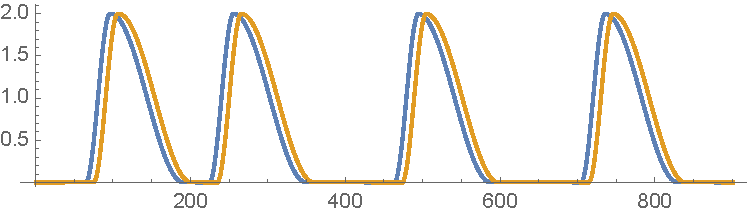
\includegraphics[width=\linewidth]{Manual/figs/tracePair.pdf}
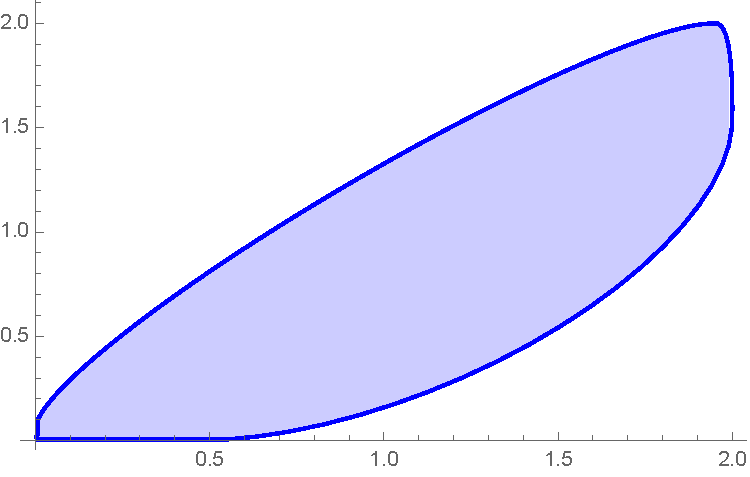
\includegraphics[width=\linewidth]{Manual/figs/area.pdf}
\caption{\small The plot on the left shows the traces of two cyclic but not periodic COOM processes modeled by the function $\gamma_k=\phi(R(\tau)-\alpha_k)$. The plot on the right shows the area between the two processes as determined by the integral $\int_I\gamma_ld\gamma_k$. This area is assigned a positive or negative value when the boundary is traced out in a counterclockwise or clockwise direction, respectively.}
\end{wrapfigure}
To measure the lead-follow relationship between processes we calculate the algebraic area between the traces which can be done using integrals of the form 
\begin{equation}
\label{eqn:integral}
A_{kl} = \oint_I\gamma_ld\gamma_k=\frac{1}{2}\oint_I\gamma_ld\gamma_k - \gamma_kd\gamma_l
\end{equation}
where $I$ is the time interval. This measures the area shown such that the area is positive if the trajectory is traced out in a counterclockwise direction, and negative if traced in a clockwise direction. This area is calculated for each pair of traces and stored in a matrix $A$, which we call the \textbf{lead matrix}.

\subsubsection{Sorting}
Assume that the function $\phi$ is noiseless and composed of a single harmonic (or is approximated by a single harmonic such as the first term of the fourier expansion). Then calculating the integral in Eq. \ref{eqn:integral} using 
$$\gamma_k(t) = a_k\phi(t - \alpha_k) = a_k\sin(t - \alpha_k),$$ 
we see that the areas in the lead matrix are given by 
$$A_{kl} = a_ka_lI\sin(\alpha_k - \alpha_l) = \frac{a_ka_lI}{2i}\left(e^{i(\alpha_k-\alpha_l)} - e^{-i(\alpha_k-\alpha_l)}\right),$$
which says that the matrix $A$ is a rank-2 matrix with basis elements
$$A_{kl}^+ = e^{i(\alpha_k - \alpha_l)} \qquad A_{kl}^- = e^{-i(\alpha_k-\alpha_l)}.$$
Note that this integral is invariant with respect to the time reparameterization, which is what allows us to work with non-periodic processes. The eigenvectors of $A$ are found by solving 
$$A_{kl}v^l = \lambda v^k.$$
Using the (+) and (-) basis elements, the eigenvectors are found to be
$$v_1 = \left(a_1e^{i\alpha_1},a_2e^{i\alpha_2},\cdots,a_ne^{i\alpha_n}\right) \qquad v_2 = \overline{v_1}$$
where $n$ is the number of processes. Hence, sorting the first eigenvector according to phase angle is the same as sorting by offset, which is how we arrive at our ordered result.

\subsection{Analyze Cyclicity}
The main function of this architecture is to analyze the cyclicity of one or multiple time series matrices. 

\end{document}